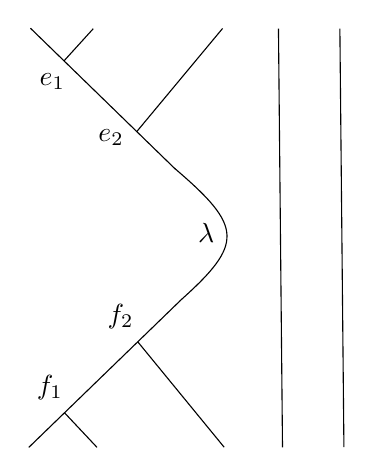
\begin{tikzpicture}[yscale=-1,scale=0.03,baseline={([yshift=-.5ex]current bounding box.center)}]
\begin{scope}[shift={(0.00mm,719.29mm)}]
% path id='path4136'
% path spec='m 158.61611,-720.41431 612.81491,595.7565'
\draw [fill=none,draw=black] (158.62mm,-720.41mm)
-- ++(612.81mm,595.76mm)
;
% path id='path4138'
% path spec='M 151.47195,1054.1879 791.4297,434.14567'
\draw [fill=none,draw=black] (151.47mm,1054.19mm)
-- (791.43mm,434.15mm)
;
% path id='path4140'
% path spec='m 769.64544,-126.57152 c 287.64226,245.969 294.60606,317.19075 20.71292,561.19558'
\draw [fill=none,draw=black] (769.65mm,-126.57mm)
.. controls ++(287.64mm,245.97mm) and ++(273.89mm,-244.00mm) .. ++(20.71mm,561.20mm)
;
% path id='path4142'
% path spec='M 301.05896,-582.61799 424.36847,-718.3111'
\draw [fill=none,draw=black] (301.06mm,-582.62mm)
-- (424.37mm,-718.31mm)
;
% path id='path4144'
% path spec='M 608.12506,-282.2081 972.02319,-719.55652'
\draw [fill=none,draw=black] (608.13mm,-282.21mm)
-- (972.02mm,-719.56mm)
;
% path id='path4146'
% path spec='M 302.57673,907.33124 440.17194,1053.7387'
\draw [fill=none,draw=black] (302.58mm,907.33mm)
-- (440.17mm,1053.74mm)
;
% path id='path4148'
% path spec='M 612.49977,606.56253 978.54075,1053.1967'
\draw [fill=none,draw=black] (612.50mm,606.56mm)
-- (978.54mm,1053.20mm)
;
% path id='path4150'
% path spec='m 1208.545,-718.87834 17.1418,1772.71524'
\draw [fill=none,draw=black] (1208.55mm,-718.88mm)
-- ++(17.14mm,1772.72mm)
;
% path id='path4152'
% path spec='m 1468.5279,-718.87834 17.1418,1772.00104'
\draw [fill=none,draw=black] (1468.53mm,-718.88mm)
-- ++(17.14mm,1772.00mm)
;
\node [black] at (902.86mm,146.65mm) { $\lambda$ };
\node [black] at (251.43mm,-496.21mm) { $e_1$ };
\node [black] at (500.14mm,-259.07mm) { $e_2$ };
\node [black] at (240.86mm,800.93mm) { $f_1$ };
\node [black] at (540.57mm,500.93mm) { $f_2$ };
\end{scope}
\end{tikzpicture}
